\documentclass[10pt,brazil,english]{article}
\usepackage{amsfonts}
\usepackage{infocomp}
\usepackage{times}
\usepackage{amsmath}
\usepackage{amssymb}
\usepackage[T1]{fontenc}
\usepackage[english, portuguese]{babel}
\addto\captionsportuguese{
\renewcommand{\figurename}{Figura}
\renewcommand{\tablename}{Tabela}
\renewcommand{\refname}{REFER\^{E}NCIAS}
}
\usepackage[utf8]{inputenc}
\usepackage{multirow}
\usepackage{lscape}
\usepackage{rotating}
\usepackage{setspace} % espacamento entre linhas
\usepackage[table,xcdraw]{xcolor}
\usepackage{scalefnt}
\usepackage{graphicx}
\usepackage{hyperref}
\usepackage{subfigure}
\usepackage{enumerate}
\usepackage{caption}
\usepackage[sort,compress]{cite}
\usepackage[alf,abnt-repeated-author-omit=yes,abnt-etal-list=0]{abntex2cite}	% Citações padrão ABNT
%%%%%%%%%%%%%%%%%%%%%%%%%%%%%%%%%%%%%%%%%%%%%%%%%%%%%%%%%
\usepackage{fancyhdr}
\usepackage{mathtools}
\setcounter{page}{1}
\fancyhead{ }
\lhead{}
\chead{\footnotesize A PREENCHER}
\rhead{}
\cfoot{}
\rfoot{\thepage}%Direita do Rodapé
\renewcommand{\headrulewidth}{1pt}% Traço horizontal no cabeçalho

%%%%%%%%%%%%%%%%%%%%%%%%%%%%%%%%%%%%%%%%%%%%%%%%%%%%%%%%%

\usepackage{rangecite}

%\hyphenation{po-pu-la-ri-za-ção re-gis-tros do-mi-na-do-ra vio-la pe-ram-bu-lam dou-tri-na-ria-men-te co-nhe-ce-rem Ad-mis-tra-ção fa-bri-car so-cie-da-de in-fe-rio-res vee-men-te-men-te si-tua-ção pon-tuais}

\sloppy
\renewcommand{\captionfont}{\footnotesize}
\renewcommand{\captionlabelfont}{\footnotesize \bfseries}
\title{ANÁLISE E IMPLEMENTAÇÃO DE MODELOS ESTOCÁSTICOS PARA EVOLUÇÃO DE ESPÉCIES}

\address{
$^{1}$Fundação Getulio Vargas (FGV)}

\author{Lucas Emanuel Resck Domingues$^{1}$}

\selectlanguage{english}

\abstract{To be filled.}

\keywords{To. Be. Filled.}

\selectlanguage{brazil}

\resumo {A preencher.}

\palchaves{A. Preencher.}

\begin{document}
    \pagestyle{fancy} % CABECALHOO
    
    \maketitle
    \newpage

    \newtheorem{theorem}{Teorema}
    
    \section{\uppercase{Introdução}}
    
    \section{\uppercase{Modelo Bak-Sneppen}}

        \citeonline{bak1993punctuated} introduziram o modelo que chamarei de Bak-Sneppen.
        Seu funcionamento é descrito de forma direta por \citeonline{khouri2013estudos}:

        \renewcommand{\theenumi}{\roman{enumi}} 
        \begin{enumerate}
            \item $N$ espécies são distribuídas em um grafo circular;
            \item A cada espécie, é associado um número, chamado \textit{\textbf{fitness}}, que é uma amostra de uma distribuição uniforme em $[0, 1]$;
            \item Em cada "rodada", o indivíduo com o menor \textit{fitness} tem seu número sorteado novamente;
            \item O mesmo se repete para seus dois vizinhos.
        \end{enumerate}

        O modelo é relativamente simples, e no artigo é sugerido que a distribuição dos \textit{fitnesses} converge para uma uniforme em $(f^*, 1]$, com $f^* \approx 2/3$.

    \section{\uppercase{Modelo GMS}}

        \citeonline{guiol2009stochastic} se basearam no modelo Bak-Sneppen para criar outro modelo, que \citeonline{khouri2013estudos} chama de GMS (as iniciais dos autores). Chamaremos assim neste trabalho. Ele é descrito:

        \renewcommand{\theenumi}{\roman{enumi}} 
        \begin{enumerate}
            \item O modelo é discreto e se inicia no conjunto vazio;
            \item A cada etapa do processo, uma espécie nasce (com probabilidade $p$) ou uma espécie morre (com probabilidade $q = 1 - p$) (se o conjunto de espécies é vazio, ele se mantém constante);
            \item Cada espécie tem associada a si um número \textit{fitness} amostrado de uma uniforme $[0, 1]$;
            \item Quando uma espécie morre, a escolhida é aquela com menor \textit{fitness} para morrer.
        \end{enumerate}

        Os autores apresentam alguns resultados. Seja $p$ tal que $p \in (1/2, 1)$ e tomemos $$f_c = \frac{1 - p}{p}\textrm{.}$$
        Então $f_c \in (0, 1)$.
        Consideremos $L_n$ e $R_n$ as espécies que estão vivas no tempo $n$ que são menores e maiores que $f_c$, respectivamente. Ou seja, $L_n \subseteq (0, f_c)$ e $R_n \subseteq (f_c, 1)$. A notação $|A|$ indica a cardinalidade de $A$. Então:

        \begin{theorem} \cite{guiol2009stochastic}
            \label{theorem1}
            \renewcommand{\theenumi}{\alph{enumi}} 
            \begin{enumerate}
                \item $|L_n|$ é uma cadeia de nascimento-morte recorrente nula. Em particular, $L_n$ é vazio infinitas vezes com probabilidade um.
                \item Se $f_c < a < b < 1$, então $$\lim_{n \to \infty} \dfrac{1}{n} |R_n \cap (a, b)| = p(b - a) \textrm{.}$$
            \end{enumerate}
        \end{theorem}

        São resultados muito fortes, porém \citeonline{guiol2009stochastic} resumem dizendo que assintoticamente a distribuição das espécies se dá uniformemente em $(f_c, 1)$.

    \section{\uppercase{Implementação}}

        A implementação dos modelos foi realizada em \textit{Python} e os resultados foram visualizados em \textit{Jupyter Notebook} \cite{domingues2019github}.

        O objetivo desta etapa é verificar os resultados apresentados que dizem respeito à convergência da distribuição dos \textit{fitnesses}.

    \section{\uppercase{Resultados}}

        \subsection{Modelo Bak-Sneppen}

            O algoritmo implementado para o modelo foi executado com 2000 espécies por 1 milhão de iterações.
            A Figura \ref{Fig1} mostra um histograma dos \textit{fitnesses}.

            \begin{figure}[!hbtp]
                \begin{center}
                    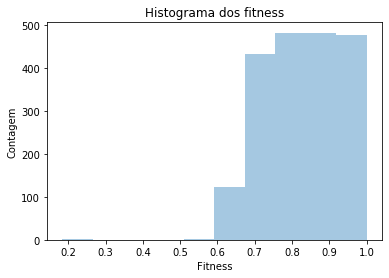
\includegraphics[scale=0.5]{Images/5-1.png}
                \end{center}
                \caption{Histograma dos \textit{fitnesses} para 2000 espécies em um milhão de iterações.}
                \label{Fig1}
            \end{figure}

        \subsection{Modelo GMS}

            O algoritmo implementado para o modelo foi executado com cem mil iterações.
            A Figura \ref{Fig2} mostra um histograma dos \textit{fitnesses} quando $p = 2/3$, e a Figura \ref{Fig3}, quando $p = 3/5$.

            \begin{figure}[!hbtp]
                \begin{center}
                    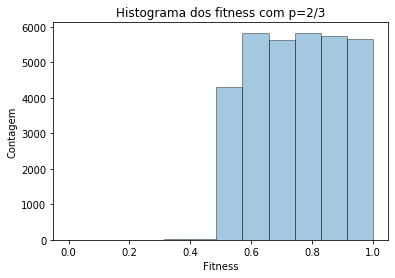
\includegraphics[scale=0.5]{Images/5-2-1.png}
                \end{center}
                \caption{Histograma dos \textit{fitnesses} para $p = 2/3$ em cem mil iterações.}
                \label{Fig2}
            \end{figure}

            \begin{figure}[!hbtp]
                \begin{center}
                    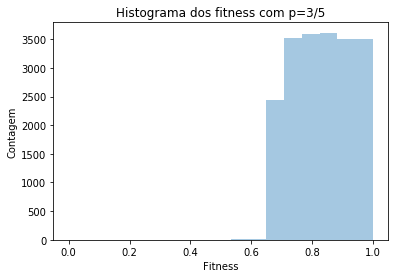
\includegraphics[scale=0.5]{Images/5-2-2.png}
                \end{center}
                \caption{Histograma dos \textit{fitnesses} para $p = 3/5$ em cem mil iterações.}
                \label{Fig3}
            \end{figure}            

    \section{\uppercase{Discussão}}

        O que ambos os modelos tentam aproximar é um processo de evolução e seleção natural.
        O modelo de Bak-Sneppen dispõe as espécies em um grafo, como uma tentativa de representar uma interação entre as espécies, como predação e comensalismo \cite{khouri2013estudos}.
        A cada rodada, a espécie menos adaptada é eliminada, de modo que surge outra espécie com \textit{fitness} aleatório, ou seja, o número de espécies é fixo.
        E o processo se repete.

        O modelo GMS adota um número de espécies variável, mas não considera interação entre as espécies.
        A não ser por essas considerações, o modelo funciona de maneira parecida: espécies surgem com \textit{fitness} aleatório e aquelas menos adaptadas morrem.

        A Figura \ref{Fig1} mostra um histograma próximo daquele de uma distribuição uniforme em $(2/3, 1]$, como é sugerido por \citeonline{bak1993punctuated}.

        A Figura \ref{Fig2} mostra um histograma próximo daquele de uma distribuição $(1/2, 1]$. Observe que $p = 2/3$.
        O Teorema \ref{theorem1} nos diz que, no limite, a distribuição das espécies é $(f_c, 1)$, com $f_c = (1 - 2/3)/(2/3) = 1/2$.
        Ora, é isso que observamos.

        Análogo à Figura \ref{Fig2}, a Figura \ref{Fig3} aproxima uma distribuição uniforme em $(2/3, 1]$, o que é esperado para valor $p = 3/5$ considerado.

        As simulações reforçam o que esperar das distribuições dos \textit{fitness} das espécies para cada modelo.

        Os modelos apresentados e testados possuem a vantagem de ser suficientemente simples (ao ponto de serem didáticos), em que evolução e seleção natural são resumidas em poucos passos de um algoritmo bem direto.
        Porém, toda essa simplicidade e didática refletem, de certa forma, erros conceituais importantes no estudo biológico.

        \citeonline{khouri2013estudos} aponta que ambos os modelos se baseiam na ideia do equilíbrio pontuado.

    \bibliography{Referencias}
    
\end{document} 